% !TeX spellcheck = en_US
\section{User settings}\label{section:user-settings}

In this chapter we will describe process of basic application configuration.\\

To configure application, go to menu in main window, choose Settings and then User settings. RUDE will open modal window. Default values are presented on image below.

\begin{figure*}[!ht] 
	\centering
	\makebox[\textwidth]{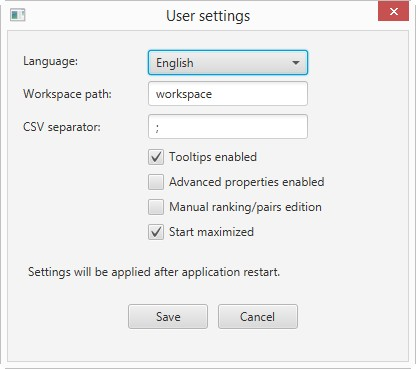
\includegraphics[width=.4\paperwidth]{raw/user-settings}}
	\caption{User settings modal dialog}
\end{figure*}


From this window you can configure following options:
\begin{itemize}
	\item \textbf{Language} - by default only English language can be chosen. Currently other languages are not supported. But you can add your own language translation, see \hyperref[sub:config-labels]{Custom language support section.}
	\item \textbf{Workspace path} - you can configure directory path for your workspace. All your projects files should be in this directory. Path is validated on form save.
	\item \textbf{CSV separator} - configures separator for csv data export. You can export data to csv in some tables by right clicking on it and selecting "Copy selected rows".
	\item \textbf{Tooltips enabled} - when this option is active, tooltips will be shown on experiment properties form with helping information.
	\item \textbf{Advanced properties enabled} - when this option is active, all experiment properties are visible on form. By default, this properties are hidden and panel needs to be expanded to access them.
	\item \textbf{Manual ranking/pairs edition} - enables manual edition of pairs and ranking on experiment properties form. It should be used only when importing manually created experiment.properties file. Application expects strict format and can not accept values with are not compatible with UI application. UI dialogs for pairs and ranking should be sufficient to configure this fields.
	\item \textbf{Start maximized} - when this option is set to true, application starts with maximum supported resolution.
\end{itemize}

All changes in configuration will be visible after application restart.


\vfill\newpage